%! Author = wolfram_e_laube
%! Date = 06.05.24

\item[(b)]
Here is a Python code snippet that accomplishes this:

\begin{verbatim}
import numpy as np
import matplotlib.pyplot as plt

# Parameters
fs = 10e3  # 10 kHz
f1 = 4e3  # 4 kHz
f2 = 6e3  # 6 kHz
frequencies = np.array([f1, f2])

# Spectrum shifting
def plot_shifted_spectrum(frequencies, fs):
    # Shift frequencies for -fs, 0, and +fs
    shifts = [-fs, 0, fs]
    shifted_freqs = [frequencies + s for s in shifts]

    plt.figure()
    for s_freqs, s in zip(shifted_freqs, shifts):
        for freq in s_freqs:
            plt.axvline(x=freq / 1e3, linestyle='-', color='b')
            plt.axvline(x=-freq / 1e3, linestyle='-', color='b')

    plt.xlabel('Frequency (kHz)')
    plt.ylabel('Amplitude')
    plt.title('Shifted Spectrum')
    plt.grid(True)
    plt.xlim(-15, 15)  # From -15 kHz to 15 kHz
    plt.show()

# Plot the shifted spectrum
plot_shifted_spectrum(frequencies, fs)
\end{verbatim}

\begin{figure}[h]
    \centering
    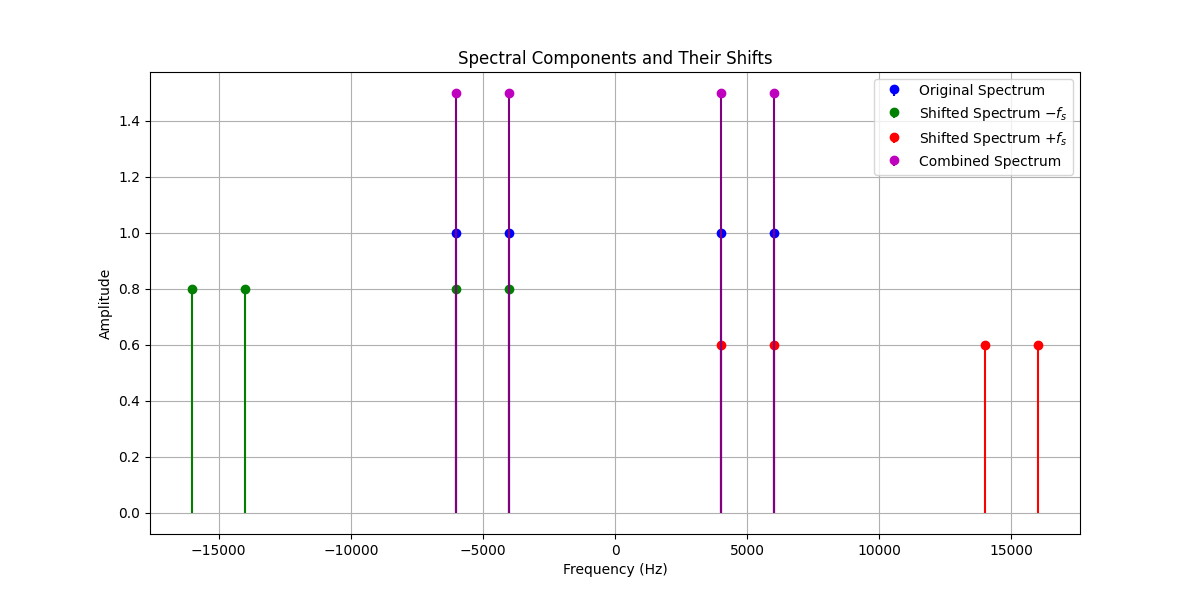
\includegraphics[width=0.49\textwidth]{fig/ex1_b_plot}
    \caption{Spectrum of \(x(t)\)}
    \label{fig:ex1_b_plot}
\end{figure}

The shifted spectrum plot will show the spectral shifts due to the sampling frequency and illustrate the overlapping spectra.